
%% Constant Velocity Questions for
%% NYSED Physics Regents Examination
%%--------------------------------------------------

%% this section contains 15 problems


%% Section June2016
%%--------------------
\element{nysed}{
\begin{question}{June2016-Q41}
    Car $A$, moving in a straight line at a constant speed of \SI{20.}{\meter\per\second},
        is initially \SI{200}{\meter} behind car $B$,
        moving in the same straight line at a constant speed of \SI{15}{\meter\per\second}. 
        How far must car $A$ travel from this initial position before it catches up with car $B$?
    \begin{multicols}{2}
    \begin{choices}
        \wrongchoice{\SI{200}{\meter}}
        \wrongchoice{\SI{800}{\meter}}
      \correctchoice{\SI{400}{\meter}}
        \wrongchoice{\SI{1000}{\meter}}
    \end{choices}
    \end{multicols}
\end{question}
}


%% Section June2015
%%--------------------
\element{nysed}{
\begin{question}{June2015-Q39}
    A car is moving with a constant speed of \SI{20}{\meter\per\second}.
    What total distance does the car travel in \SI{2.0}{\minute}?
    \begin{multicols}{2}
    \begin{choices}
        \wrongchoice{\SI{10}{\meter}}
        \wrongchoice{\SI{40}{\meter}}
        \wrongchoice{\SI{1200}{\meter}}
      \correctchoice{\SI{2400}{\meter}}
    \end{choices}
    \end{multicols}
\end{question}
}


%% Section June2012
%%--------------------
\element{nysed}{
\begin{question}{June2012-Q01}
    In a drill during basketball practice,
        a player runs the length of the \SI{30}{\meter} court and back.
    The player does this three times in \SI{60}{\second}.
    \begin{center}
        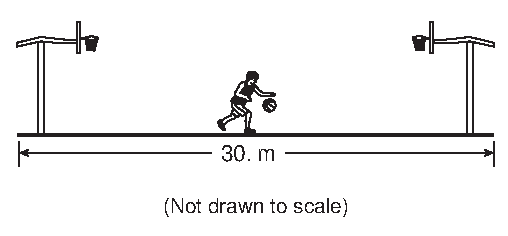
\includegraphics[keepaspectratio,scale=0.75]{June2012-Q01}
    \end{center}
    The magnitude of the player's total displacement after running the drill is:
    \begin{multicols}{2}
    \begin{choices}
      \correctchoice{\SI{0.0}{\meter}}
        \wrongchoice{\SI{30}{\meter}}
        \wrongchoice{\SI{60}{\meter}}
        \wrongchoice{\SI{180}{\meter}}
    \end{choices}
    \end{multicols}
\end{question}
}

\element{nysed}{
\begin{question}{June2012-Q02}
    In a drill during basketball practice,
        a player runs the length of the \SI{30}{\meter} court and back.
    The player does this three times in \SI{60}{\second}.
    \begin{center}
        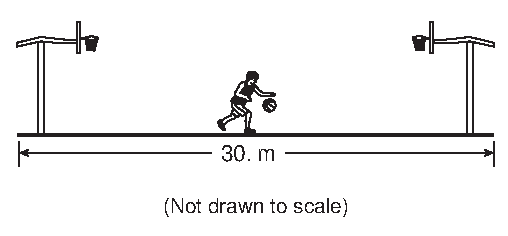
\includegraphics[keepaspectratio,scale=0.75]{June2012-Q01}
    \end{center}
    The average speed of the player during the drill is:
    \begin{multicols}{2}
    \begin{choices}
        \wrongchoice{\SI{0.0}{\meter\per\second}}
        \wrongchoice{\SI{0.50}{\meter\per\second}}
      \correctchoice{\SI{3.0}{\meter\per\second}}
        \wrongchoice{\SI{30}{\meter\per\second}}
    \end{choices}
    \end{multicols}
\end{question}
}


%% Section June2011
%%--------------------


%% Section June2010
%%--------------------
\element{nysed}{
\begin{question}{June2010-Q01}
    A baseball player runs \SI{27.4}{\meter} from the batter's box to first base,
        overruns first base by \SI{3.0}{\meter},
        and then returns to first base.
    Compared to the total distance traveled by the player,
        the magnitude of the player's total displacement from the batter's box is?
    \begin{multicols}{2}
    \begin{choices}
        \wrongchoice{\SI{3.0}{\meter} shorter}
      \correctchoice{\SI{6.0}{\meter} shorter}
        \wrongchoice{\SI{3.0}{\meter} longer}
        \wrongchoice{\SI{6.0}{\meter} longer}
    \end{choices}
    \end{multicols}
\end{question}
}


%% Section June2009
%%--------------------
\element{nysed}{
\begin{question}{June2009-Q01}
    On a highway, a car is driven \SI{80}{\kilo\meter} during the first \SI{1.00}{\hour} of travel,
        \SI{50}{\kilo\meter} during the next \SI{0.50}{\hour},
        and \SI{40}{\kilo\meter} in the final \SI{0.50}{\hour}.
    What is the car's average speed for the entire trip?
    \begin{multicols}{2}
    \begin{choices}
        \wrongchoice{\SI{45}{\kilo\meter\per\hour}}
        \wrongchoice{\SI{60}{\kilo\meter\per\hour}}
      \correctchoice{\SI{85}{\kilo\meter\per\hour}}
        \wrongchoice{\SI{170}{\kilo\meter\per\hour}}
    \end{choices}
    \end{multicols}
\end{question}
}

\element{nysed}{
\begin{question}{June2009-Q04}
    A high-speed train in Japan travels a distance of \SI{300}{\kilo\meter} in \SI{3.60e3}{\second}.
    What is the average speed of this train?
    \begin{multicols}{2}
    \begin{choices}
        \wrongchoice{\SI{1.20e-2}{\meter\per\second}}
        \wrongchoice{\SI{8.33e-2}{\meter\per\second}}
        \wrongchoice{\SI{12.0}{\meter\per\second}}
      \correctchoice{\SI{83.3}{\meter\per\second}}
    \end{choices}
    \end{multicols}
\end{question}
}


%% Section Jan2009
%%--------------------


%% Section June2008
%%--------------------
\element{nysed}{
\begin{question}{June2008-Q04}
    Approximately how much time does it take light to travel from Sun to Earth?
    \begin{multicols}{2}
    \begin{choices}
        \wrongchoice{\SI{2.00e-3}{\second}}
        \wrongchoice{\SI[retain-zero-exponent]{1.28e0}{\second}}
      \correctchoice{\SI{5.00e2}{\second}}
        \wrongchoice{\SI{4.50e19}{\second}}
    \end{choices}
    \end{multicols}
\end{question}
}


%% Section Jan2008
%%--------------------


%% Section June2007
%%--------------------


%% Section Jan2007
%%--------------------


%% Section June2006
%%--------------------


%% Section Jan2006
%%--------------------


%% Section June2005
%%--------------------


%% Section Jan2005
%%--------------------
\element{nysed}{
\begin{question}{Jan2005-Q02}
    In a \SI{4.0}{\kilo\meter} race, a runner completes the first kilometer in \SI{5.9}{\minute},
        the second kilometer in \SI{6.2}{\minute}, and the third kilometer in \SI{6.3}{\minute},
        and the final kilometer in \SI{6.0}{\minute}.
    The average speed of the runner for the race is approximately:
    \begin{multicols}{2}
    \begin{choices}
      \correctchoice{\SI{0.16}{\kilo\meter\per\minute}}
        \wrongchoice{\SI{0.33}{\kilo\meter\per\minute}}
        \wrongchoice{\SI{12}{\kilo\meter\per\minute}}
        \wrongchoice{\SI{24}{\kilo\meter\per\minute}}
    \end{choices}
    \end{multicols}
\end{question}
}


%% Section June2004
%%--------------------


%% Section Jan2004
%%--------------------


%% Section June2003
%%--------------------


%% Section Jan2003
%%--------------------


%% Section Aug2002
%%--------------------


%% Section June2002
%%--------------------


%% Section Jan2002
%%--------------------
\element{nysed}{
\begin{question}{Jan2002-Q03}
    A group of bike riders took a \SI{4.0}{\hour} trip.
    During the first \SI{3.0}{\hour},
        they traveled a total of \SI{50}{\kilo\meter},
        but during the last hour they traveled only \SI{10}{\kilo\meter}.
    What was the group's average speed for the entire trip?
    \begin{multicols}{2}
    \begin{choices}
      \correctchoice{\SI{15}{\kilo\meter\per\hour}}
        \wrongchoice{\SI{30}{\kilo\meter\per\hour}}
        \wrongchoice{\SI{40}{\kilo\meter\per\hour}}
        \wrongchoice{\SI{60}{\kilo\meter\per\hour}}
    \end{choices}
    \end{multicols}
\end{question}
}


%% Section June2001
%%--------------------
\element{nysed}{
\begin{question}{June2001-Q09}
    Two cars, $A$ and $B$, are \SI{400}{\meter} apart.
    Car $A$ travels due east at \SI{30}{\meter\per\second} on a collision course with car $B$,
        which travels due west at \SI{20}{\meter\per\second}.
    How much time elapses before the two cars collide?
    \begin{multicols}{2}
    \begin{choices}
      \correctchoice{\SI{8.0}{\second}}
        \wrongchoice{\SI{20}{\second}}
        \wrongchoice{\SI{13}{\second}}
        \wrongchoice{\SI{40}{\second}}
    \end{choices}
    \end{multicols}
\end{question}
}

\element{nysed}{
\begin{question}{June2001-Q53}
    A softball player leaves the batter's box,
        overruns first base by \SI{3.0}{\meter},
        and then returns to first base.
    Compared to the total distance traveled by the player,
        the magnitude of the player's total displacement from the batter's box is:
    \begin{multicols}{3}
    \begin{choices}
      \correctchoice{smaller}
        \wrongchoice{larger}
        \wrongchoice{the same}
    \end{choices}
    \end{multicols}
\end{question}
}


%% Section Jan2001
%%--------------------


%% Section June2000
%%--------------------


%% Section June1999
%%--------------------


%% Section June1998
%%--------------------
\element{nysed}{
\begin{question}{June1998-Q05}
    What is the average velocity of a car that travels \SI{30}{\kilo\meter} due west in \SI{0.50}{\hour}?
    \begin{multicols}{2}
    \begin{choices}
        \wrongchoice{\SI{15}{\kilo\meter\per\hour}}
        \wrongchoice{\SI{60}{\kilo\meter\per\hour}}
        \wrongchoice{\SI{15}{\kilo\meter\per\hour} west}
      \correctchoice{\SI{60}{\kilo\meter\per\hour} west}
    \end{choices}
    \end{multicols}
\end{question}
}


%% Section June1997
%%--------------------
\element{nysed}{
\begin{question}{June1997-Q02}
    A baseball pitcher throws a fastball at \SI{42}{\meter\per\second}.
    If the batter is \SI{18}{\meter} from the pitcher,
        approximately how much time does it take for the ball to reach the batter?
    \begin{multicols}{2}
    \begin{choices}
        \wrongchoice{\SI{1.0}{\second}}
        \wrongchoice{\SI{2.3}{\second}}
        \wrongchoice{\SI{0.86}{\second}}
      \correctchoice{\SI{0.43}{\second}}
    \end{choices}
    \end{multicols}
\end{question}
}


%% Section June1996
%%--------------------
\element{nysed}{
\begin{question}{June1996-Q01}
    A car travels between the \SI{100}{\meter} and \SI{250}{\meter} highway markers in \SI{10}{\second}.
    The average speed of the car during this interval is:
    \begin{multicols}{2}
    \begin{choices}
        \wrongchoice{\SI{10}{\meter\per\second}}
      \correctchoice{\SI{15}{\meter\per\second}}
        \wrongchoice{\SI{25}{\meter\per\second}}
        \wrongchoice{\SI{35}{\meter\per\second}}
    \end{choices}
    \end{multicols}
\end{question}
}


%% Section June1994
%%--------------------
\element{nysed}{
\begin{question}{June1994-Q44}
    The distance from the Moon to Earth is \SI{3.9e8}{\meter}.
    What is the time required for a light ray to travel from the Moon to Earth?
    \begin{multicols}{2}
    \begin{choices}
        \wrongchoice{\SI{0.65}{\second}}
      \correctchoice{\SI{1.3}{\second}}
        \wrongchoice{\SI{2.6}{\second}}
        \wrongchoice{\SI{3.9}{\second}}
    \end{choices}
    \end{multicols}
\end{question}
}


%% Section June1986
%%--------------------
\element{nysed}{
\begin{question}{June1986-Q02}
    The average speed of a plane was \SI{600}{\kilo\meter\per\hour}.
    How long did it take the plane to travel \SI{120}{\kilo\meter}?
    \begin{multicols}{2}
    \begin{choices}
      \correctchoice{\SI{0.2}{\hour}}
        \wrongchoice{\SI{0.5}{\hour}}
        \wrongchoice{\SI{0.7}{\hour}}
        \wrongchoice{\SI{5}{\hour}}
    \end{choices}
    \end{multicols}
\end{question}
}

\element{nysed}{
\begin{question}{June1986-Q19}
    It takes \SI{1}{\second} for a sound wave to travel from a source to observer $A$.
    How long does it take the same sound wave to travel in the same medium to observer $B$,
        who is located twice as far from the source as observer $A$?
    \begin{multicols}{4}
    \begin{choices}
        \wrongchoice{\SI{1/4}{\second}}
      \correctchoice{\SI{2}{\second}}
        \wrongchoice{\SI{1/2}{\second}}
        \wrongchoice{\SI{4}{\second}}
    \end{choices}
    \end{multicols}
\end{question}
}


%% Section June1985
%%--------------------
\element{nysed}{
\begin{question}{June1985-Q02}
    The distance-time graph below represents the position of an object moving in a straight line.
    \begin{center}
    \begin{tikzpicture}
        \begin{axis}[
            axis y line=left,
            axis x line=bottom,
            axis line style={->},
            xlabel={time},
            x unit=\si{\second},
            xtick={0,1,2,3,4,5,6},
            minor x tick num=1,
            ylabel={distance},
            y unit=\si{\meter},
            ytick={0,10,20,30},
            minor y tick num=1,
            xmin=0,xmax=6.3,
            ymin=0,ymax=31.5,
            width=0.8\columnwidth,
            height=0.5\columnwidth,
            grid=major,
            very thin,
        ]
        \addplot[line width=1pt,mark=\empty] plot coordinates { (0,0) (2,10) (4,30) (6,30)};
        \end{axis}
    \end{tikzpicture}
    \end{center}
    What is the speed of the object during the time interval $t=\SI{2.0}{\second}$ to $t=\SI{4.0}{\second}$?
    \begin{multicols}{2}
    \begin{choices}
        \wrongchoice{\SI{0.0}{\meter\per\second}}
        \wrongchoice{\SI{5.0}{\meter\per\second}}
        \wrongchoice{\SI{7.5}{\meter\per\second}}
      \correctchoice{\SI{10.}{\meter\per\second}}
    \end{choices}
    \end{multicols}
\end{question}
}


\endinput


